\documentclass[a4paper,12pt]{article}
\usepackage{amsmath, bm}
\usepackage{amssymb, amsthm, graphicx}
\usepackage{enumitem}
\usepackage{color}
\usepackage{float}
\usepackage[small]{caption}
\usepackage{subcaption}
\usepackage[mathscr]{euscript}
\usepackage{dsfont}
\usepackage{natbib}
\usepackage{amsmath}
\usepackage{placeins}
\usepackage{rotating}
\usepackage{pdflscape}
\makeatletter
\renewcommand{\eqref}[1]{\tagform@{\ref{#1}}}
\def\maketag@@@#1{\hbox{#1}}
\makeatother
\usepackage{bibentry}
\usepackage[left=2.7cm, right=2.7cm, bottom=2.7cm, top=2.7cm]{geometry}
%\parindent0pt 
\newcommand{\doublehat}[1]{\skew{5.5}\widehat{\widehat{#1}}}
\newcommand{\doublehattwo}[1]{\widehat{\widehat{#1}}}



% General

\newcommand{\reals}{\mathbb{R}}
\newcommand{\integers}{\mathbb{Z}}
\newcommand{\naturals}{\mathbb{N}}

\newcommand{\pr}{\mathbb{P}}        % probability
\newcommand{\ex}{\mathbb{E}}        % expectation
\newcommand{\var}{\textnormal{Var}} % variance
\newcommand{\cov}{\textnormal{Cov}} % covariance

\newcommand{\law}{\mathcal{L}} % law of X
\newcommand{\normal}{N}        % normal distribution 

\newcommand{\argmax}{\textnormal{argmax}}
\newcommand{\argmin}{\textnormal{argmin}}

\newcommand{\ind}{\mathbbm{1}} % indicator function
\newcommand{\kernel}{K} % kernel function
\newcommand{\wght}{W} % kernel weight
\newcommand{\thres}{\pi} % threshold parameter


% Convergence

\newcommand{\convd}{\stackrel{d}{\longrightarrow}}              % convergence in distribution
\newcommand{\convp}{\stackrel{P}{\longrightarrow}}              % convergence in probability
\newcommand{\convas}{\stackrel{\textrm{a.s.}}{\longrightarrow}} % convergence almost surely
\newcommand{\convw}{\rightsquigarrow}                           % weak convergence


% Theorem-like declarations

\theoremstyle{plain}

\newtheorem{theorem}{Theorem}[section]
\newtheorem{prop}[theorem]{Proposition}
\newtheorem{lemma}[theorem]{Lemma}
\newtheorem{corollary}[theorem]{Corollary}
\newtheorem*{theo}{Theorem}
\newtheorem{propA}{Proposition}[section]
\newtheorem{lemmaA}[propA]{Lemma}
\newtheorem{definition}{Definition}[section]
\newtheorem{remark}{Remark}[section]
\renewcommand{\thelemmaA}{A.\arabic{lemmaA}}
\renewcommand{\thepropA}{A.\arabic{propA}}
\newtheorem*{algo}{Clustering Algorithm}


% Theorem numbering to the left

\makeatletter
\newcommand{\lefteqno}{\let\veqno\@@leqno}
\makeatother


% Heading

\newcommand{\heading}[2]
{  \setcounter{page}{1}
   \begin{center}

   \phantom{Distance to upper boundary}
   \vspace{0.5cm}

   {\LARGE \textbf{#1}}
   \vspace{0.4cm}
 
   {\LARGE \textbf{#2}}
   \end{center}
}


% Authors

\newcommand{\authors}[4]
{  \parindent0pt
   \begin{center}
      \begin{minipage}[c][2cm][c]{5cm}
      \begin{center} 
      {\large #1} 
      \vspace{0.05cm}
      
      #2 
      \end{center}
      \end{minipage}
      \begin{minipage}[c][2cm][c]{5cm}
      \begin{center} 
      {\large #3}
      \vspace{0.05cm}

      #4 
      \end{center}
      \end{minipage}
   \end{center}
}

%\newcommand{\authors}[2]
%{  \parindent0pt
%   \begin{center}
%   {\large #1} 
%   \vspace{0.1cm}
%      
%   #2 
%   \end{center}  
%}


% Version

\newcommand{\version}[1]
{  \begin{center}
   {\large #1}
   \end{center}
   \vspace{3pt}
} 










\begin{document}

\section{State of the art and preliminary work}\label{sec-intro}


The comparison of nonparametric curves is a classic topic in econometrics and statistics. Depending on the specific application, the curves of interest are densities, distribution functions, time trends or regression curves. The problem of testing for equality of densities has been studied in \cite{Mammen1992}, \cite{Anderson1994} and \cite{Li2009} among others. Tests for equality of distribution functions can be found for example in \cite{Kiefer1959}, \cite{Anderson1962} and \cite{Finner2018}. Tests for equality of trend or regression curves have been developed in \cite{HaerdleMarron1990}, \cite{Hall1990}, \cite{Delgado1993}, \cite{DegrasWu2012}, \cite{Zhang2012} and \cite{Hidalgo2014} among many others. In the proposed project, we focus on the comparison of nonparametric trend curves.


The statistical problem of comparing trends has a wide range of applications in economics, finance and other fields such as climatology and biology. In economics, one may wish is to compare trends in real gross domestic product (GDP) across different countries \citep[cp.][]{Grier1989}. Another example concerns the dynamics of long-term interest rates. To better understand these dynamics, researchers aim to compare the yields of US Treasury bills at different maturities over time \citep[cp.][]{Park2009}. In finance, it is of interest to compare the volatility trends of different stocks \citep[cp.][]{Nyblom2000}. Finally, in climatology, researchers are interested in comparing the trending behaviour of temperature time series across different spatial locations \citep[cp.][]{KarolyWu2005}. 


Classically, time trends are modelled stochastically in econometrics; see e.g.\ \cite{Stock1988}. Recently, however, there has been a growing interest in econometric models with deterministic time trends; see \cite{Cai2007}, \cite{Atak2011}, \cite{Robinson2012} and \cite{ChenGaoLi2012} among others. Non- and semiparametric trend modelling has attracted particular interest in a panel data context. \cite{LiChenGao2010}, \cite{Atak2011}, \cite{Robinson2012} and \cite{ChenGaoLi2012} considered panel models where the observed time series have a common time trend. In many applications, however, the assumption of a common time trend is quite harsh. In particular when the number of observed time series is large, it is quite natural to suppose that the time trend may differ across time series. More flexible panel settings with heterogeneous trends have been studied, for example, in \cite{Zhang2012} and \cite{Hidalgo2014}. 

 
In what follows, we consider a general panel framework with heterogeneous trends which is useful for a number of economic and financial applications: Suppose we observe a panel of $n$ time series $\mathcal{Z}_i = \{ (Y_{it},\mathbf{X}_{it}): 1 \le t \le T \}$ for $1 \le i \le n$, where $Y_{it}$ are real-valued random variables and $\mathbf{X}_{it} = (X_{it,1},\ldots,X_{it,d})^\top$ are $d$-dimensional random vectors. Each time series $\mathcal{Z}_i$ is modelled by the equation
\begin{equation}\label{model}
Y_{it} = m_i \Big( \frac{t}{T} \Big) + \bm{\beta}_i^\top \mathbf{X}_{it} + \alpha_i + \varepsilon_{it}
\end{equation}
for $1 \le t \le T$, where $m_i: [0,1] \rightarrow \mathbb{R}$ is a nonparametric (deterministic) trend function, $\mathbf{X}_{it}$ is a vector of regressors or controls and $\bm{\beta}_i$ is the corresponding parameter vector. Moreover, $\alpha_i$ are so-called fixed effect error terms and $\varepsilon_{it}$ are standard regression errors with $\ex[\varepsilon_{it}|\mathbf{X}_{it}] = 0$ for all $t$. Model \eqref{model} nests a number of panel models which have recently been considered in the literature. Special cases of model \eqref{model} with a nonparametric trend specification are for example considered in \cite{Atak2011}, \cite{Zhang2012} and \cite{Hidalgo2014}. Versions of model \eqref{model} with a parametric trend are studied in \cite{Vogelsang2005}, \cite{Sun2011} and \cite{Xu2012} among others.

Within the general framework of model \eqref{model}, we can formulate a number of interesting statistical questions concerning the set of trend functions $\{ m_i:  1 \le i \le n \}$. 

\vspace{10pt}


\noindent \textbf{(a) Testing for equality of nonparametric trend curves} 
\vspace{10pt} 

 
\noindent In many application contexts, an important question is whether the time trends $m_i$ in model \eqref{model} are all the same. Put differently, the question is whether the observed time series
have a common trend. This question can formally be addressed by a statistical test of the null hypothesis 
\[ H_0: \text{There exists a function } m: [0,1] \rightarrow \mathbb{R} \text{ such that } m_i = m  \text{ for all } 1 \le i \le n. \]
A closely related question is whether all time trends have the same parametric form. To formulate the corresponding null hypothesis, let $m(\theta,\cdot): [0,1] \rightarrow \mathbb{R}$ be a function which is known up to the finite-dimensional parameter $\theta \in \Theta$, where $\Theta$ denotes the parameter space. The null hypothesis of interest now reads as follows:  
\[ H_{0,\text{para}}: \text{ There exists } \theta \in \Theta \text{ such that } m_i(\cdot) = m(\theta,\cdot) \text{ for all } 1 \le i \le n. \]  
If $m(\theta,w) = a + b w$ with $\theta = (a,b)$, for example, then $H_0$ is the hypothesis that all trends $m_i$ are linear with the same intercept $a$ and slope $b$. A somewhat simpler but yet important hypothesis is given by 
\[ H_{0,\text{const}}: m_i \equiv 0 \text{ for all } 1 \le i \le n. \]
Under this hypothesis, there is no time trend at all in the observed time series. Put differently, all the time trends $m_i$ are constant. (Note that under the normalization constraint $\int_0^1 m_i(w) dw = 0$, $m_i$ must be equal to zero if it is a constant function.) A major goal of our project is to develop new tests for the hypotheses $H_0$, $H_{0,\text{para}}$ and $H_{0,\text{const}}$ in model \eqref{model}. In order to keep the exposition as clear as possible, we focus attention on the hypothesis $H_0$ in what follows. Tests of $H_{0,\text{para}}$, $H_{0,\text{const}}$ and related hypotheses have for example been studied in \cite{Lyubchich2016} and \cite{ChenWu2018}. 


In recent years, a number of different approaches have been developed to test the hypothesis $H_0$. \cite{DegrasWu2012} consider the problem of testing $H_0$ within the model framework
\begin{equation}\label{model-degras}
Y_{it} = m_i \Big( \frac{t}{T} \Big) + \alpha_i + \varepsilon_{it} \qquad (1 \le t \le T, \, 1 \le i \le n), 
\end{equation}
where $\mathbb{E}[\varepsilon_{it}] = 0$ for all $i$ and $t$ and the terms $\alpha_i$ are assumed to be deterministic. Obviously, \eqref{model-degras} is a special case of \eqref{model} which does not include additional regressors. \cite{DegrasWu2012} construct an $L_2$-type statistic to test $H_0$. The statistic is based on the difference between estimators of the trend with and without imposing $H_0$. Let $\hat{m}_{i,h}$ be the estimator of $m_i$ and $\hat{m}_h$ the estimator of the common trend $m$ under $H_0$, where $h$ denotes the bandwidth parameter. With these estimators, the authors define the statistic
\begin{equation}\label{stat-degras}
\Delta_{n,T} = \sum_{i=1}^n \int_0^1 \big(\hat{m}_{i,h}(u) - \hat{m}_h(u)\big)^2 du, 
\end{equation} 
which measures the $L_2$-distance between $\hat{m}_{i, h}$ and $\hat{m}_h$. In the theoretical part of their paper, they derive the limit distribution of $\Delta_{n,T}$. \cite{ChenWu2018} develop theory for test statistics closely related to those from \cite{DegrasWu2012}, but under more general conditions on the error terms. 


\cite{Zhang2012} investigate the problem of testing the hypothesis $H_0$ in a slightly restricted version of model \eqref{model}, where $\beta_i = \beta$ for all $i$. The regression coefficients $\beta_i$ are thus assumed to be homogeneous in their setting. They construct a residual-based test statistic as follows: First, they obtain profile least squares estimators $\hat{\beta}$ and $\hat{m}_h(t/T)$ of the parameter vector $\beta$ and the common trend $m$ under $H_0$, where $h$ denotes the bandwidth. With these estimators, they compute the residuals $\hat{u}_{it} = Y_{it} - \hat{\beta}^T X_{it} - \hat{m}_h(t/T)$. These residuals are shown to have the form $\hat{u}_{it} = \Delta_i(t/T) + \eta_{it}$, where $\Delta_i$ is a deterministic function with the property that $\Delta_i \equiv 0$ under $H_0$ and $\eta_{it}$ denotes the error term. Testing $H_0$ is thus equivalent to testing the hypothesis $H_0^\prime: \Delta_i \equiv 0$ for all $1 \le i \le n$. The authors construct a test statistic for the hypothesis $H_0^\prime$ on the basis of nonparametric kernel estimators of the functions $\Delta_i$ and derive its limit distribution.  


The tests of \cite{Zhang2012}, \cite{DegrasWu2012} and \cite{ChenWu2018} are based on nonparametric estimators of the trend functions $m_i$ that depend on one or several bandwidth parameters. Unfortunately, it is far from clear how to choose these bandwidths in an appropriate way. This is a general problem concerning essentially all tests based on nonparametric curve estimators. There are of course many theoretical results on optimal bandwidth choice for estimation purposes. However, the optimal bandwidth for curve estimation is usually not optimal for testing. Optimal bandwidth choice for tests is indeed an open problem, and only little theory for simple cases is available \citep[cp.][]{GaoGijbels2008}. Since tests based on nonparametric curve estimators are commonly quite sensitive to the choice of bandwidth and theory for optimal bandwidth selection is not available, it appears preferable to work with bandwidth-free tests. 


A classical way to obtain a bandwidth-free test of the hypothesis $H_0$ is to use CUSUM-type statistics which are based on partial sum processes. This approach is taken in \cite{Hidalgo2014}. A more modern approach to obtain a bandwidth-free test is to employ multiscale methods. These methods avoid the need to choose a bandwidth by considering a large collection of bandwidths simultaneously. More specifically, the basic idea is as follows: Let $S_h$ be a test statistic for the null hypothesis of interest, which depends on the bandwidth $h$. Rather than considering only a single statistic $S_h$ for a specific bandwidth $h$, a multiscale approach simultaneously considers a whole family of statistics $\{S_h: h \in \mathcal{H} \}$, where $\mathcal{H}$ is a set of bandwidth values. The multiscale test then proceeds as follows: For each bandwidth or scale $h$, one checks whether $S_h > q_h(\alpha)$, where $q_h(\alpha)$ is a bandwidth-dependent critical value (for given significance level $\alpha$). The multiscale test rejects if $S_h > q_h(\alpha)$ for at least one scale $h$. The main theoretical difficulty in this approach is of course to derive appropriate critical values $q_h(\alpha)$. Specifically, the critical values $q_h(\alpha)$ need to be determined such that the multiscale test has the correct (asymptotic) level, that is, such that $\pr (S_h > q_h(\alpha) \text{ for some } h \in \mathcal{H} ) = (1-\alpha) + o(1)$. 


Multiscale methods have been developed for a variety of different test problems in recent years. \cite{ChaudhuriMarron1999, ChaudhuriMarron2000} introduced the so-called SiZer method which has been extended in various directions; see for example \cite{HannigMarron2006} and \cite{Rondonotti2007}. \cite{HorowitzSpokoiny2001} proposed a multiscale test for the parametric form of a regression function. \cite{DuembgenSpokoiny2001} constructed a multiscale approach which works with additively corrected supremum statistics. This general approach has been very influential in recent years and has been further developed in numerous ways; see for example \cite{Duembgen2002}, \cite{Rohde2008} and \cite{ProkschWernerMunk2018} for multiscale methods in the regression context and \cite{DuembgenWalther2008}, \cite{RufibachWalther2010}, \cite{SchmidtHieber2013} and \cite{EckleBissantzDette2017} for methods in the context of density estimation. Importantly, all of these studies are restricted to the case of independent data. It turns out that it is highly non-trivial to extend the multiscale approach of \cite{DuembgenSpokoiny2001} to the case of dependent data. A first step into this direction has recently been made in \cite{KhismatullinaVogt2020}. They developed multiscale methods to test for local increases/decreases of the nonparametric trend function $m$ in the univariate time series model $Y_t = m(t/T) + \varepsilon_t$.  


To the best of our knowledge, multiscale tests of the hypotheses $H_0$, $H_{0,\text{para}}$ and $H_{0,\text{const}}$ in model \eqref{model} are not available in the literature. The only exception is \cite{Park2009} who developed SiZer methods for the comparison of nonparametric trend curves in a strongly simplified version of model \eqref{model}. Their analysis, however, is mainly methodological and not fully backed up by theory. Indeed, theory has only been derived for the special case $n=2$, that is, for the case that only two time series are observed. 
\vspace{10pt}


\noindent \textbf{(b) Clustering of nonparametric trend curves} 
\vspace{10pt} 


\noindent Consider the situation that the null hypothesis $H_0: m_1 = \ldots = m_n$ is violated in the general panel data model \eqref{model}. Even though some of the trend functions $m_i$ are different in this case, there may still be groups of time series with the same time trend. Formally, a group stucture can be defined as follows within the framework of model \eqref{model}: There exist sets or groups of time series $G_1,\ldots,G_{K_0}$ with $\{1,\ldots,n\} = \dot\bigcup_{k=1}^{K_0} G_k$ such that for each $1 \le k \le K_0$, 
\begin{equation}\label{model-groups}
m_i = m_j \quad \text{for all } i,j \in G_k. 
\end{equation}
According to \eqref{model-groups}, the time series of a given group $G_k$ all have the same time trend. In many applications, it is very natural to suppose that there is such a group structure in the data. An interesting statistical problem which we aim to investigate in our project is how to estimate the unknown groups $G_1,\ldots,G_{K_0}$ and their unknown number $K_0$ from the data. 


Several approaches to this problem have been proposed in the context of models closely related to \eqref{model}. \cite{DegrasWu2012} used a repeated testing procedure based on $L_2$-type test statistics of the form \eqref{stat-degras} in order to estimate the unknown group structure in model \eqref{model-degras}. \cite{Zhang2013} developed a clustering method within the same model framework which makes use of an extended Bayesian information criterion. \cite{VogtLinton2017} constructed a thresholding method to estimate the unknown group structure in the panel model $Y_{it} = m_i(X_{it}) + u_{it}$, where $X_{it}$ are random regressors and $u_{it}$ are general error terms that may include fixed effects. Their approach can also be adapted to the case of fixed regressors $X_{it} = t/T$.  As an alternative to a group structure, factor-type structures have been imposed on the trend and regression functions in panel models. Such factor-type structures are studied in \cite{Kneip2012}, \cite{LintonVogt2015} and \cite{BonevaLintonVogt2016} among others. 


The problem of estimating the unknown groups $G_1,\ldots,G_{K_0}$ and their unknown number $K_0$ in model \eqref{model} has close connections to functional data clustering. There, the aim is to cluster smooth random curves that are functions of (rescaled) time and that are observed with or without noise. A number of different clustering approaches have been proposed in the context of functional data models; see for example \cite{Abraham2003}, \cite{Tarpey2003} and \cite{Tarpey2007} for procedures based on $k$-means clustering, \cite{James2003} and \cite{Chiou2007} for model-based clustering approaches and \cite{Jacques2014} for a recent survey. 


The problem of finding the unknown group structure in model \eqref{model} is also closely related to a developing literature in econometrics which aims to identify unknown group structures in parametric panel regression models. In its simplest form, the panel regression model under consideration is given by the equation $Y_{it} = \beta_i^\top X_{it} + u_{it}$ for $1 \le t \le T$ and $1 \le i \le n$, where the coefficient vectors $\beta_i$ are allowed to vary across individuals $i$ and the error terms $u_{it}$ may include fixed effects. Similar to the trend functions in model \eqref{model}, the coefficients $\beta_i$ are assumed to belong to a number of groups: there are $K_0$ groups $G_1,\ldots,G_{K_0}$ such that $\beta_i = \beta_j$ for all $i,j \in G_k$ and all $1\le k \le K_0$. The problem of estimating the unknown groups and their unknown number has been studied in different versions of this modelling framework; cp.\ \cite{Su2016}, \cite{Su2018} and \cite{Wang2018} among others. \cite{Bonhomme2015} considered a related model where the group structure is not imposed on the regression coefficients but rather on some unobserved time-varying fixed effect components of the panel model. 


Virtually all the proposed procedures to cluster nonparametric curves in panel and functional data models related to \eqref{model} depend on a number of bandwidth or smoothing parameters required to estimate the nonparametric functions $m_i$. In general, nonparametric curve estimators are strongly affected by the chosen bandwidth parameters. A clustering procedure which is based on such estimators can be expected to be strongly influenced by the choice of bandwidths as well. Moreover, as in the context of statistical testing, there is no theory available on how to pick the bandwidths optimally for the clustering problem. Hence, as in the context of testing, it is desirable to construct a clustering procedure which is free of bandwidth or smoothing parameters that need to be selected. 


One way to obtain a clustering method which does not require to select any bandwidth parameter is to use multiscale methods. This approach has recently been taken in \cite{VogtLinton2018}. They develop a clustering approach in the context of the panel model $Y_{it} = m_i(X_{it}) + u_{it}$, where $X_{it}$ are random regressors and $u_{it}$ are general error terms that may include fixed effects. Imposing the same group structure as in \eqref{model-groups} on their  model, they construct estimators of the unknown groups and their unknown number as follows: In a first step, they develop bandwidth-free multiscale statistics $\hat{d}_{ij}$ which measure the distance between pairs of functions $m_i$ and $m_j$. To construct them, they make use of the multiscale testing methods described in part (a) of this section. In a second step, the statistics $\hat{d}_{ij}$ are employed as dissimilarity measures in a hierarchical clustering algorithm. 


\section{The model}\label{sec-model}

The model setting is as follows. We observe time series $\mathcal{Y}_i = \{Y_{it}: 1 \le t \le T \}$ of length $T$ for $1 \le i \le n$. Each time series $\mathcal{Y}_i$ satisfies the model equation \begin{equation}\label{model_full}
Y_{it} = \beta^\prime X_{it} + m_i \Big( \frac{t}{T} \Big) + \alpha_i + \varepsilon_{it} 
\end{equation}
for $1 \le t \le T$, where $\beta$ is a $d \times 1$ vector of unknown parameters, $X_{it}$ is a $d\times 1$ vector of individual covariates, $m_i$ is an unknown nonparametric trend function defined on $[0,1]$, $\alpha_i$ is a (deterministic or random) intercept term and $\mathcal{E}_i = \{ \varepsilon_{it}: 1 \le t \le T \}$ is a zero-mean stationary error process. For identification, we normalize the functions $m_i$ such that $\int_0^1 m_i(u) du = 0$ for all $1 \le i \le n$. The term $\alpha_i$ can also be regarded as an additional error component. In the econometrics literature, it is commonly called a fixed effect error term. It can be interpreted as capturing unobserved characteristics of the time series $\mathcal{Y}_i$ which remain constant over time. We allow the error terms $\alpha_i$ to be dependent across $i$ in an arbitrary way. Hence, by including them in model equation \eqref{model_full}, we allow the $n$ time series $\mathcal{Y}_i$ in our sample to be correlated with each other. Whereas the terms $\alpha_i$ may be correlated, the error processes $\mathcal{E}_i$ are assumed to be independent across $i$. In addition, each process $\mathcal{E}_i$ is supposed to satisfy the conditions \ref{C-err1}--\ref{C-err3}. Finally note that throughout the paper, we restrict attention to the case where the number of time series $n$ in model \eqref{model} is fixed. Extending our theoretical results to the case where $n$ slowly grows with the sample size $T$ is a possible topic for further research.

The stationary error processes $\{\varepsilon_{it}\}_{t\in\integers}$ are assumed to have the following properties: 
\begin{enumerate}[label=(C\arabic*),leftmargin=1.05cm]

\item \label{C-err1} For each $i$ the variables $\varepsilon_{it}$ allow for the representation $\varepsilon_{it} = G_i(\ldots,\eta_{it-1},\eta_{it},\eta_{it+1},\ldots)$, where $\eta_{it}$ are i.i.d.\ random variables across $t$ and $G_i: \reals^\integers \rightarrow \reals$ is a measurable function. Denote $Eta_{it} = i(\ldots,\eta_{it-1},\eta_{it})$.

\item \label{C-err2} It holds that $\ex[\varepsilon_{it}] =0$ and $\| \varepsilon_{it} \|_q < \infty$ for some $q > 4$, where $\| \varepsilon_{it} \|_q = (\ex|\varepsilon_t|^q)^{1/q}$. 

\end{enumerate}

Following \cite{Wu2005}, we impose conditions on the dependence structure of the error process $\{\varepsilon_{it}\}_{t\in\integers}$ in terms of the physical dependence measure $d_{i, t,q} = \| \varepsilon_{it} - \varepsilon_{it}^\prime \|_q$, where $\varepsilon_{it}^\prime = G(\ldots,\eta_{i(-1)},\eta_{i0}^\prime,\eta_{i1},\ldots,\eta_{it-1},\eta_{it},\eta_{it+1},\ldots)$ with $\{\eta_{it}^\prime\}$ being an i.i.d.\ copy of $\{\eta_{it}\}$. In particular, we assume the following: 
\begin{enumerate}[label=(C\arabic*),leftmargin=1.05cm]
\setcounter{enumi}{2}

\item \label{C-err3} Define $\Theta_{i, t,q} = \sum\nolimits_{|s| \ge t} d_{i, s,q}$ for $t \ge 0$. It holds that 
$\Theta_{i, t,q} = O ( t^{-\tau_q} (\log t)^{-A} )$,  
where $A > \frac{2}{3} (1/q + 1 + \tau_q)$ and $\tau_q = \{q^2 - 4 + (q-2) \sqrt{q^2 + 20q + 4}\} / 8q$. 

\end{enumerate}
The conditions \ref{C-err1}--\ref{C-err3} are fulfilled by a wide range of stationary processes $\{\varepsilon_{it}\}_{t\in\integers}$.%As a first example, consider linear processes of the form $\varepsilon_t = \sum\nolimits_{i=0}^{\infty} c_i \eta_{t-i}$ with $\| \varepsilon_t \|_q < \infty$, where $c_i$ are absolutely summable coefficients and $\eta_t$ are i.i.d.\ innovations with $\ex[\eta_t] = 0$ and $\| \eta_t\|_q < \infty$. Trivially, \ref{C-err1} and \ref{C-err2} are fulfilled in this case. Moreover, if $|c_i| = O(\rho^i)$ for some $\rho \in (0,1)$, then \ref{C-err3} is easily seen to be satisfied as well. As a special case, consider an ARMA process $\{\varepsilon_t\}$ of the form $\varepsilon_t - \sum\nolimits_{i=1}^p a_i \varepsilon_{t-i} = \eta_t + \sum\nolimits_{j=1}^r b_j \eta_{t-j}$  with $\| \varepsilon_t \|_q < \infty$, where $a_1,\ldots,a_p$ and $b_1,\ldots,b_r$ are real-valued parameters. As before, we let $\eta_t$ be i.i.d.\ innovations with $\ex[\eta_t] = 0$ and $\| \eta_t\|_q < \infty$. Moreover, as usual, we suppose that the complex polynomials $A(z) = 1 - \sum\nolimits_{j=1}^p a_jz^j$ and $B(z) = 1 + \sum\nolimits_{j=1}^r b_jz^j$ do not have any roots in common. If $A(z)$ does not have any roots inside the unit disc, then the ARMA process $\{ \varepsilon_t \}$ is stationary and causal. Specifically, it has the representation $\varepsilon_t = \sum\nolimits_{i=0}^{\infty} c_i \eta_{t-i}$ with $|c_i| = O(\rho^i)$ for some $\rho \in (0,1)$, implying that \ref{C-err1}--\ref{C-err3} are fulfilled. The results in \cite{WuShao2004} show that condition \ref{C-err3} (as well as the other two conditions) is not only fulfilled for linear time series processes but also for a variety of non-linear processes. 


\section{Testing for equality of time trends}\label{sec-test-equality}

In this section, we adapt the multiscale method developed in Section \ref{sec-method} to test the hypothesis that the trend functions in model \eqref{model} are all the same. More formally, we test the null hypothesis $H_0: m_1 = m_2 = \ldots = m_n$ in model \eqref{model_full}. As we will see, the proposed multiscale method does not only allow to test whether the null hypothesis is violated. It also provides information on where violations occur. More specifically, it allows to identify, with a pre-specified confidence, (i) trend functions which are different from each other and (ii) time intervals where these trend functions differ.


%\subsection{Construction of the test statistic in the absence of exogenous regressors}\label{subsec-test-equality-stat-without-regs}
%
%As a starting point we will first provide a test for common trends in the absence of exogenous covariates $X_{it}$. So we begin with a model
%\begin{equation}\label{model}
%Y_{it} = m_i \Big( \frac{t}{T} \Big) + \alpha_i + \varepsilon_{it},
%\end{equation} 
%where $\varepsilon_{it}$ are zero-mean error terms and $\alpha_i$ are (random or deterministic) intercepts. Defining $Y_{it}^\circ = Y_{it} - \alpha_i$, this equation can be rewritten as $Y_{it}^\circ = m_i(\frac{t}{T}) + \varepsilon_{it}$, which is a standard nonparametric regression equation. The variables $Y_{it}^\circ$ are not observed, but they can be approximated by $\widehat{Y}_{it} = Y_{it} - \widehat{\alpha}_i$, where $\widehat{\alpha}_i = T^{-1} \sum_{t=1}^T Y_{it}$ is an estimator of the intercept $\alpha_i$. By construction, $\widehat{\alpha}_i - \alpha_i = T^{-1} \sum_{t=1}^T \varepsilon_{it} + T^{-1} \sum_{t=1}^T m_i(\frac{t}{T}) = O_p(T^{-1/2}) + T^{-1} \sum_{t=1}^T m_i(\frac{t}{T})$. Hence, $\widehat{\alpha}_i$ is a reasonable estimator of $\alpha_i$ if $T^{-1} \sum_{t=1}^T m_i(\frac{t}{T})$ converges to zero as $T \rightarrow \infty$. To ensure this, we suppose throughout the section that the functions $m_i$ are Lipschitz continuous, that is, $|m_i(v) - m_i(w)| \le L|v - w|$ for all $v,w \in [0,1]$ and some constant $L < \infty$. Since $\int_0^1 m_i(u) du = 0$ by normalization, this implies that $T^{-1} \sum_{t=1}^T m_i(\frac{t}{T}) = O(T^{-1})$. We further let $\widehat{\sigma}_i^2$ be an estimator of the long-run error variance $\sigma_i^2 = \sum\nolimits_{\ell=-\infty}^{\infty} \cov(\varepsilon_{i0}, \varepsilon_{i\ell})$ which is computed from the constructed sample $\{ \widehat{Y}_{it}: 1 \le t \le T \}$. We thus regard $\widehat{\sigma}_i^2 = \widehat{\sigma}_i^2(\widehat{Y}_{i1},\ldots,\widehat{Y}_{iT})$ as a function of the variables $\widehat{Y}_{it}$ for $1 \le t \le T$. Throughout the section, we assume that $\widehat{\sigma}_i^2 = \sigma_i^2 + o_p(\rho_T)$ with $\rho_T = o(1/\log T)$. Details on how to construct estimators of $\sigma_i^2$ are deferred to Section \ref{sec-error-var}. 
%
%
%We are now ready to introduce the multiscale statistic for testing the hypothesis $H_0: m_1 = m_2 = \ldots = m_n$. For any pair of time series $i$ and $j$, we define the kernel averages
%\[ \widehat{\psi}_{ij,T}(u,h) = \sum\limits_{t=1}^T w_{t,T}(u,h)(\widehat{Y}_{it} - \widehat{Y}_{jt}), \]
%where the kernel weights $w_{t,T}(u,h)$ are defined as in \eqref{weights}. The kernel average $\widehat{\psi}_{ij,T}(u,h)$ can be regarded as measuring the distance between the two trend curves $m_i$ and $m_j$ on the interval $[u-h,u+h]$. Similar as in Section \ref{subsec-method-stat}, we aggregate the kernel averages $\widehat{\psi}_{ij,T}(u,h)$ for all $(u,h) \in \mathcal{G}_T$ by the multiscale statistic 
%\[ \widehat{\Psi}_{ij,T} = \max_{(u,h) \in \mathcal{G}_T} \Big\{ \Big|\frac{\widehat{\psi}_{ij,T}(u,h)}{(\widehat{\sigma}_i^2 + \widehat{\sigma}_j^2)^{1/2}}\Big| - \lambda(h) \Big\}, \] 
%where $\lambda(h) = \sqrt{2 \log \{ 1/(2h) \}}$ and the set $\mathcal{G}_T$ has been introduced in Section \ref{subsec-method-stat}. The statistic $\widehat{\Psi}_{ij,T}$ can be interpreted as a distance measure between the two curves $m_i$ and $m_j$. We finally define the multiscale statistic for testing the null hypothesis $H_0: m_1 =m_2 = \ldots = m_n$ as
%\[ \widehat{\Psi}_{n,T} = \max_{1 \le i < j \le n} \widehat{\Psi}_{ij,T}, \]
%that is, we define it as the maximal distance $\widehat{\Psi}_{ij,T}$ between any pair of curves $m_i$ and $m_j$ with $i \ne j$. 
%
%
%\subsection{The test procedure}\label{subsec-test-equality-test}
%
%
%Let $Z_{it}$ for $1 \le t \le T$ and $1 \le i \le n$ be independent standard normal random variables which are independent of the error terms $\varepsilon_{it}$. Denote the empirical average of the variables $Z_{i1},\ldots,Z_{iT}$ by $\bar{Z}_{i,T} = T^{-1} \sum_{t=1}^T Z_{it}$. To simplify notation, we write $\bar{Z}_i = \bar{Z}_{i,T}$ in what follows. For each $i$ and $j$, we introduce the Gaussian statistic 
%\[ \Phi_{ij,T} = \max_{(u,h) \in \mathcal{G}_T} \Big\{ \Big|\frac{\phi_{ij,T}(u,h)}{(\widehat{\sigma}_i^2 + \widehat{\sigma}_j^2)^{1/2}}\Big| - \lambda(h) \Big\}, \] 
%where $\phi_{ij,T}(u,h) = \sum\nolimits_{t=1}^T w_{t,T}(u,h) \, \{ \widehat{\sigma}_i (Z_{it} - \bar{Z}_i) - \widehat{\sigma}_j (Z_{jt} - \bar{Z}_j) \}$. Moreover, we define the statistic
%\[ \Phi_{n,T} = \max_{1 \le i < j \le n} \Phi_{ij,T} \]
%and denote its $(1-\alpha)$-quantile by $q_{n,T}(\alpha)$. Our multiscale test of the hypothesis $H_0: m_1 = m_2 = \ldots = m_n$ is defined as follows: For a given significance level $\alpha \in (0,1)$, we reject $H_0$ if $\widehat{\Psi}_{n,T} > q_{n,T}(\alpha)$. 
%
%
%\subsection{Theoretical properties of the test}\label{subsec-test-equality-theo}
%
%
%To start with, we introduce the auxiliary statistic 
%\[ \widehat{\Phi}_{n,T} = \max_{1 \le i < j \le n} \widehat{\Phi}_{ij,T}, \]
%where
%\[ \widehat{\Phi}_{ij,T} = \max_{(u,h) \in \mathcal{G}_T} \Big\{ \Big| \frac{\widehat{\phi}_{ij,T}(u,h)} {\{ \widehat{\sigma}_i^2 + \widehat{\sigma}_j^2 \}^{1/2}} \Big| - \lambda(h) \Big \} \]
%and $\widehat{\phi}_{ij,T}(u,h) = \sum_{t=1}^T w_{t,T}(u,h) \{ (\varepsilon_{it} - \bar{\varepsilon}_i) - (\varepsilon_{jt} - \bar{\varepsilon}_j) \}$ with $\bar{\varepsilon}_i = \bar{\varepsilon}_{i,T} = T^{-1} \sum_{t=1}^T \varepsilon_{it}$. Our first theoretical result characterizes the asymptotic behaviour of the statistic $\widehat{\Phi}_{n,T}$ and parallels Theorem \ref{theo-stat} from Section \ref{sec-method}. 
%\begin{theorem}\label{theo-stat-equality}
%Suppose that the error processes $\mathcal{E}_i = \{ \varepsilon_{it}: 1 \le t \le T \}$ are independent across $i$ and satisfy \ref{C-err1}--\ref{C-err3} for each $i$. Moreover, let \ref{C-ker}--\ref{C-h} be fulfilled and assume that $\widehat{\sigma}_i^2 = \sigma_i^2 + o_p(\rho_T)$ with $\rho_T = o(1/\log T)$ for each $i$. Then 
%\[ \pr \big( \widehat{\Phi}_{n,T} \le q_{n,T}(\alpha) \big) = (1 - \alpha) + o(1). \]
%\end{theorem}
%Theorem \ref{theo-stat-equality} is the main stepping stone to derive the theoretical properties of our multiscale test. It can be proven by slightly modifying the arguments for Theorem \ref{theo-stat}. The details are provided in the Supplementary Material. The following proposition characterizes the behaviour of our multiscale test under the null hypothesis and under local alternatives. 
%\begin{prop}\label{prop-test-equality}
%Let the conditions  of Theorem \ref{theo-stat-equality} be satisfied. 
%\begin{enumerate}[label=(\alph*),leftmargin=0.75cm]
%\item Under the null hypothesis $H_0: m_1 = m_2 = \ldots = m_n$, it holds that 
%\[ \pr \big( \widehat{\Psi}_{n,T} \le q_{n,T}(\alpha) \big) = (1 - \alpha) + o(1). \]
%\item Let $m_i = m_{i,T}$ be a Lipschitz continuous function with $\int_0^1 m_{i,T}(w) dw = 0$ for any $i$. In particular, suppose that $|m_{i,T}(v) - m_{i,T}(w)| \le L |v - w|$ for all $v,w \in [0,1]$ and some fixed constant $L < \infty$ which does not depend on $T$. Moreover, assume that for some pair of indices $i$ and $j$, the functions $m_{i,T}$ and $m_{j,T}$ have the following property: There exists $(u,h) \in \mathcal{G}_T$ with $[u-h,u+h] \subseteq [0,1]$ such that $m_{i,T}(w) - m_{j,T}(w) \ge c_T \sqrt{\log T/(Th)}$ for all $w \in [u-h,u+h]$ or $m_{j,T}(w) - m_{i,T}(w) \ge c_T \sqrt{\log T/(Th)}$ for all $w \in [u-h,u+h]$, where $\{c_T\}$ is any sequence of positive numbers with $c_T \rightarrow \infty$. Then 
%\[ \pr \big( \widehat{\Psi}_{n,T} \le q_{n,T}(\alpha) \big) = o(1). \]
%\end{enumerate}
%\end{prop}
%Part (a) of Proposition \ref{prop-test-equality} is a direct consequence of Theorem \ref{theo-stat-equality}. The proof of part (b) is very similar to that of Proposition \ref{prop-test-2} and thus omitted. 
%
%

\subsection{Construction of the test statistic in the presence of exogenous regressors}\label{subsec-test-equality-stat-with-regs}

We now extend the model \eqref{model} to include the exogenous regressors:
\begin{equation}
Y_{it} = \beta_i^\prime X_{it} + m_i \Big( \frac{t}{T} \Big) + \alpha_i + \varepsilon_{it} 
\end{equation}
It is obvious that if $\beta_i$ is known, the problem of testing for the common time trend would be reduced to the one discussed before. That is, we would test $H_0: m_1 = m_2 = \ldots = m_n$ in the model
\begin{align*}
Y_{it} - \beta_i^\prime X_{it} & =: V_{it}\\
					& = m_i \Big( \frac{t}{T} \Big) + \alpha_i + \varepsilon_{it} 
\end{align*}
replacing $Y_{it}$ by $V_{it}$ in the construction of the test statistic. However, $\beta_i$ is not known so we need to estimate it first. Given an estimator $\widehat{\beta}_i$, we then consider
\begin{align*}
	\widehat{V}_{it} := Y_{it} - \widehat{\beta}_i^\prime X_{it} =(\widehat{\beta}_i - \beta_i)^\prime X_{it} + m_i \Big( \frac{t}{T} \Big) + \alpha_i + \varepsilon_{it} 
\end{align*}
and construct the kernel averages $\widehat{\psi}_{ij, T}(u, h)$ based on $\widehat{V}_{it}$ instead of $\widehat{Y}_{it}$. Specifically, for any pair of time series $i$ and $j$ we define the kernel averages
\begin{align*}
	\widehat{\psi}^{\prime}_{ij, T}(u, h) = \sum_{t=1}^T w_{t, T}(u, h)(\widehat{V}_{it} - \widehat{V}_{jt})
\end{align*}
with the kernel weights defined in ??. Similar as in Section \ref{subsec-test-equality-stat-without-regs}, we aggregate the kernel averages $\widehat{\psi}^{\prime}_{ij, T}(u, h)$ for all $(u, h)\in \mathcal{G}_T$ by the multiscale test statistic
\[ \widehat{\Psi}^\prime_{ij,T} = \max_{(u,h) \in \mathcal{G}_T} \Big\{ \Big|\frac{\widehat{\psi}^\prime_{ij,T}(u,h)}{(\widehat{\sigma}_i^2 + \widehat{\sigma}_j^2)^{1/2}}\Big| - \lambda(h) \Big\}. \]

We now focus on finding an appropriate estimator $\widehat{\beta}$ of $\beta$. For that purpose, we consider the time series $\{\Delta Y_{it}\}$ of the differences $\Delta Y_{it} = Y_{it} - Y_{i t-1}$ for each $i$. We then have
\begin{align*}
	\Delta Y_{it} = Y_{it} - Y_{i t-1} =\beta_i^\prime \Delta X_{it} + \bigg(m_i \Big( \frac{t}{T} \Big) - m_i \Big(\frac{t-1}{T}\Big)\bigg) + \Delta \varepsilon_{it},
\end{align*}
where $\Delta X_{it} = X_{it} - X_{it-1}$ and $ \Delta \varepsilon_{it} = \varepsilon_{it} - \varepsilon_{i t-1}$. Since $m_i(\cdot)$ is Lipschitz, we can use the fact that $ \big|m_i \big( \frac{t}{T} \big) - m_i \big(\frac{t-1}{T}\big) \big| = O\big(\frac{1}{T}\big)$ and rewrite 
\begin{align*}
	\Delta Y_{it} = \beta_i^\prime \Delta X_{it} + \Delta \varepsilon_{it} + O\Big(\frac{1}{T}\Big).
\end{align*}

For a class of stochastic processes $\{\mathbf{L}(v, \mathcal{F}_t)\}_{t\in\integers}$, we say that the process is $\mathcal{L}^q$ \textit{stochastic Lipschitz-continuous} over $[0,1]$ if
\[ \sup_{0\leq v_1 < v_2 \leq 1} \frac{||\mathbf{L}(v_2, \mathcal{F}_0) - \mathbf{L}(v_1, \mathcal{F}_0)||_q}{|v_2 - v_1|} < \infty.
\]
We denote the collection of $\mathcal{L}^q$ \textit{stochastic Lipschitz-continuous} over $[0,1]$ classes by $Lip_q$.

\subsection{Nonstationary regressors}

We need the following assumptions on the independent variables $X_{it}$ for each $i$:

\begin{enumerate}[label=(C\arabic*),leftmargin=1.05cm]
\setcounter{enumi}{3}

\item \label{C-reg1} The covariates $X_{it}$ allow for the representation $X_{it} = \mathbf{H}_i(t/T, \mathcal{U}_{it})$, where $\mathcal{U}_{it} =(\ldots,u_{it-1},u_{it})$ with $u_{it}$ being i.i.d.\ random variables and $\mathbf{H}_i := (H_{i1}, H_{i2}, \ldots, H_{id})^T: [0, 1] \times \reals^\integers \rightarrow \reals^d$ is a measurable function such that $\mathbf{H}_i(v, \mathcal{U}_{it})$ is well defined for each $v\in [0,1]$. 

\item \label{C-reg2} Let $N_i(v)$ be the $d\times d$ matrix with $kl$-th entry $n_{i, kl}(v) = \ex[H_{ik}(v, \mathcal{U}_{i0}), H_{il}(v, \mathcal{U}_{i0})]$. We assume that the smallest eigenvalue of $N_i(v)$ is bounded away from $0$ on $v\in[0,1]$.

\item \label{C-reg3} Let $\mathbf{H}_{i}(v, \mathcal{U}_{it}) \in Lip_2$ and $\sup_{0\leq v\leq 1}||\mathbf{H}_{i}(v, \mathcal{U}_{it})||_4 <\infty$.
\end{enumerate}

We define the first-differenced regressors as follows.
\[ \Delta \mathbf{X}_{it} =\mathbf{H}_i(v_t, \mathcal{U}_{it}) - \mathbf{H}_i(v_{t-1}, \mathcal{U}_{it-1}) := \Delta \mathbf{H}_i(v_t, \mathcal{U}_{it}) \]
where $v_t = t/T$. Similarly, 
\[\Delta \varepsilon_{it} = \varepsilon_{it} - \varepsilon_{it-1} = G_i(\ldots, \eta_{it-1}, \eta_{it}) - G_i(\ldots, \eta_{it-2}, \eta_{it-1}) = \Delta G_i(\ldots, \eta_{it-1}, \eta_{it}).
\]
 
With these assumptions we can prove the following proposition.
\begin{prop}\label{prop-reg-1}
Under Assumptions \ref{C-reg1} - \ref{C-reg3},
\[ \Delta \mathbf{H}_i(v_t, \mathcal{U}_{it}) \in Lip_2 \text{ and } \sup_{0\leq v \leq 1} || \Delta \mathbf{H}_i(v, \mathcal{U}_{it})||_4 < \infty
\]
\end{prop}

\begin{proof}[\textnormal{\textbf{Proof of Proposition \ref{prop-reg-1}}}]
Note the following 
\begin{align*}
&\sup_{0\leq v_t < v_s \leq 1} \frac{||\Delta \mathbf{H}_i(v_s, \mathcal{U}_{i0}) - \Delta \mathbf{H}_i(v_t, \mathcal{U}_{i0}) ||_2}{|v_s - v_t|} \leq \\
\leq &\sup_{0\leq v_t < v_s \leq 1} \frac{||\mathbf{H}_i(v_s, \mathcal{U}_{i0}) - \mathbf{H}_i(v_{s-1}, \mathcal{U}_{i0}) - |\mathbf{H}_i(v_t, \mathcal{U}_{i0}) - \mathbf{H}_i(v_{t-1}, \mathcal{U}_{i0})| ||_2}{|v_s - v_t|} \leq\\
\leq &\sup_{0\leq v_t < v_s \leq 1} \frac{||\mathbf{H}_i(v_s, \mathcal{U}_{i0}) - \mathbf{H}_i(v_t, \mathcal{U}_{i0}) ||_2}{|v_s - v_t|} + \sup_{0\leq v_{t-1} < v_{s-1} \leq 1} \frac{||\mathbf{H}_i(v_{s-1}, \mathcal{U}_{i0}) - \mathbf{H}_i(v_{t-1}, \mathcal{U}_{i0}) ||_2}{|v_{s-1} - v_{t-1}|},
\end{align*}
where $v_s - v_t = v_{s-1} - v_{t-1}$ by definition. By Assumption \ref{C-reg3},
\[\sup_{0\leq v_t < v_s \leq 1} \frac{||\mathbf{H}_i(v_s, \mathcal{U}_{i0}) - \mathbf{H}_i(v_t, \mathcal{U}_{i0}) ||_2}{|v_s - v_t|} < \infty
\]
and 
\[\sup_{0\leq v_{t-1} < v_{s-1} \leq 1} \frac{||\mathbf{H}_i(v_{s-1}, \mathcal{U}_{i0}) - \mathbf{H}_i(v_{t-1}, \mathcal{U}_{i0}) ||_2}{|v_{s-1} - v_{t-1}|} < \infty.
\]
Thus, 
\[
\sup_{0\leq v_t < v_s \leq 1} \frac{||\Delta \mathbf{H}_i(v_s, \mathcal{U}_{i0}) - \Delta \mathbf{H}_i(v_t, \mathcal{U}_{i0}) ||_2}{|v_s - v_t|} < \infty
\]
and $\Delta \mathbf{H}_i(v_t, \mathcal{U}_{it}) \in Lip_2$. Moreover, by Assumption \ref{C-reg3},
\[
 \sup_{0\leq v_t \leq 1} || \Delta \mathbf{H}_i(v_t, \mathcal{U}_{it})||_4 \leq  \sup_{0\leq v_t \leq 1} ||\mathbf{H}_i(v, \mathcal{U}_{it})||_4 +  \sup_{0\leq v_{t-1} \leq 1} || \mathbf{H}_i(v_{t-1}, \mathcal{U}_{it-1})||_4 < \infty,
\]
which completes the proof.
\end{proof} 

To be able to prove the next proposition, we need an additional assumption on the relationship between the covariates and the error process.

\begin{enumerate}[label=(C\arabic*),leftmargin=1.05cm]
\setcounter{enumi}{6}
\item \label{C-reg4} For each $i$ $\{\eta_{it}\}_{t\in\integers}$ from Assumption \ref{C-err1} and $\{u_{it}\}_{t\in\integers}$ from Assumption \ref{C-reg1} are independent of each other.
\end{enumerate}


\begin{prop}\label{prop-reg-2}
Under Assumptions \ref{C-err1} - \ref{C-reg4},
\[ \Big| \frac{1}{\sqrt{T}}\sum_{t=1}^T \Delta \mathbf{X}_{it}\Delta \varepsilon_{it} \Big| = O_P(1)
\]
\end{prop}
\begin{proof}[\textnormal{\textbf{Proof of Proposition \ref{prop-reg-2}}}]
Let $\zeta_{i,t} = (u_{i, t}, \eta_{i, t})^T$. We need the following notation:
\begin{alignat*}{2}
&\mathcal{I}_{i,t} &&:= (\ldots, \zeta_{i, t-2}, \zeta_{i, t-1}, \zeta_{i,t}),\\
&\Delta \mathbf{U}_i(v, \mathcal{I}_{i, t}) &&:= \Delta \mathbf{H}_i(v_t, \mathcal{U}_{it}) \Delta G_i(\ldots, \eta_{it-1}, \eta_{it}),\\
&\mathcal{P}_{i,t}(\cdot) &&:= \ex[\cdot|\mathcal{I}_{i, t}] -\ex[\cdot|\mathcal{I}_{i, t-1}], \\
&\kappa_{i} && := \frac{1}{T}\sum_{t=1}^T  \Delta \mathbf{X}_{it}\Delta \varepsilon_{it}, \\
&\kappa_{i, s}^{\mathcal{P}} && := \frac{1}{T}\sum_{t=1}^T \mathcal{P}_{i, t-s}\big( \Delta \mathbf{X}_{it}\Delta \varepsilon_{it}\big).
\end{alignat*}
Then,
\begin{align*}
||\kappa_{i, s}^{\mathcal{P}}||^2 &= \Big|\Big| \frac{1}{T}\sum_{t=1}^T \mathcal{P}_{i, t-s}\big( \Delta \mathbf{X}_{it}\Delta \varepsilon_{it}\big) \Big|\Big|^2 \leq\\
&\leq \frac{1}{T^2} \sum_{t=1}^T \Big|\Big| \ex (\Delta \mathbf{X}_{it}\Delta \varepsilon_{it}|\mathcal{I}_{i, t-s}) -\ex (\Delta \mathbf{X}_{it}\Delta \varepsilon_{it}|\mathcal{I}_{i, t-s-1}) \Big|\Big|^2 =\\
&= \frac{1}{T^2} \sum_{t=1}^T \Big|\Big| \ex (\Delta \mathbf{X}_{it}\Delta \varepsilon_{it}|\mathcal{I}_{i, t-s}) -\ex (\Delta \mathbf{X}_{it, s}^*\Delta \varepsilon_{it, s}^*|\mathcal{I}_{i, t-s}) \Big|\Big|^2,
\end{align*}
where $\Delta \mathbf{X}_{it, s}^*\Delta \varepsilon_{it, s}^*$ denotes $\Delta \mathbf{X}_{it}\Delta \varepsilon_{it}$ with $\zeta_{i, t-s}$ replaced by its i.i.d. copy $\zeta_{i, t-s}^*$. In this case $\ex (\Delta \mathbf{X}_{it, s}^*\Delta \varepsilon_{it, s}^*|\mathcal{I}_{i, t-s -1}) = \ex (\Delta \mathbf{X}_{it, s}^*\Delta \varepsilon_{it, s}^*|\mathcal{I}_{i, t-s})$. Furthermore, by linearity of the expectation and Jensen's inequality we have 
\begin{align*}
||\kappa_{i, s}^{\mathcal{P}}||^2 &\leq \frac{1}{T^2} \sum_{t=1}^T \Big|\Big| \ex (\Delta \mathbf{X}_{it}\Delta \varepsilon_{it}|\mathcal{I}_{i, t-s}) -\ex (\Delta \mathbf{X}_{it, s}^*\Delta \varepsilon_{it, s}^*|\mathcal{I}_{i, t-s}) \Big|\Big|^2 \leq \\
&\leq \frac{1}{T^2} \sum_{t=1}^T \Big|\Big| \Delta \mathbf{X}_{it}\Delta \varepsilon_{it} -\Delta \mathbf{X}_{it, s}^*\Delta \varepsilon_{it, s}^*\Big|\Big|^2
\end{align*}

\end{proof}

\subsection{Analysis of UK weather station data}\label{subsec-data-2} 

%\begin{figure}[t]
%\centering
%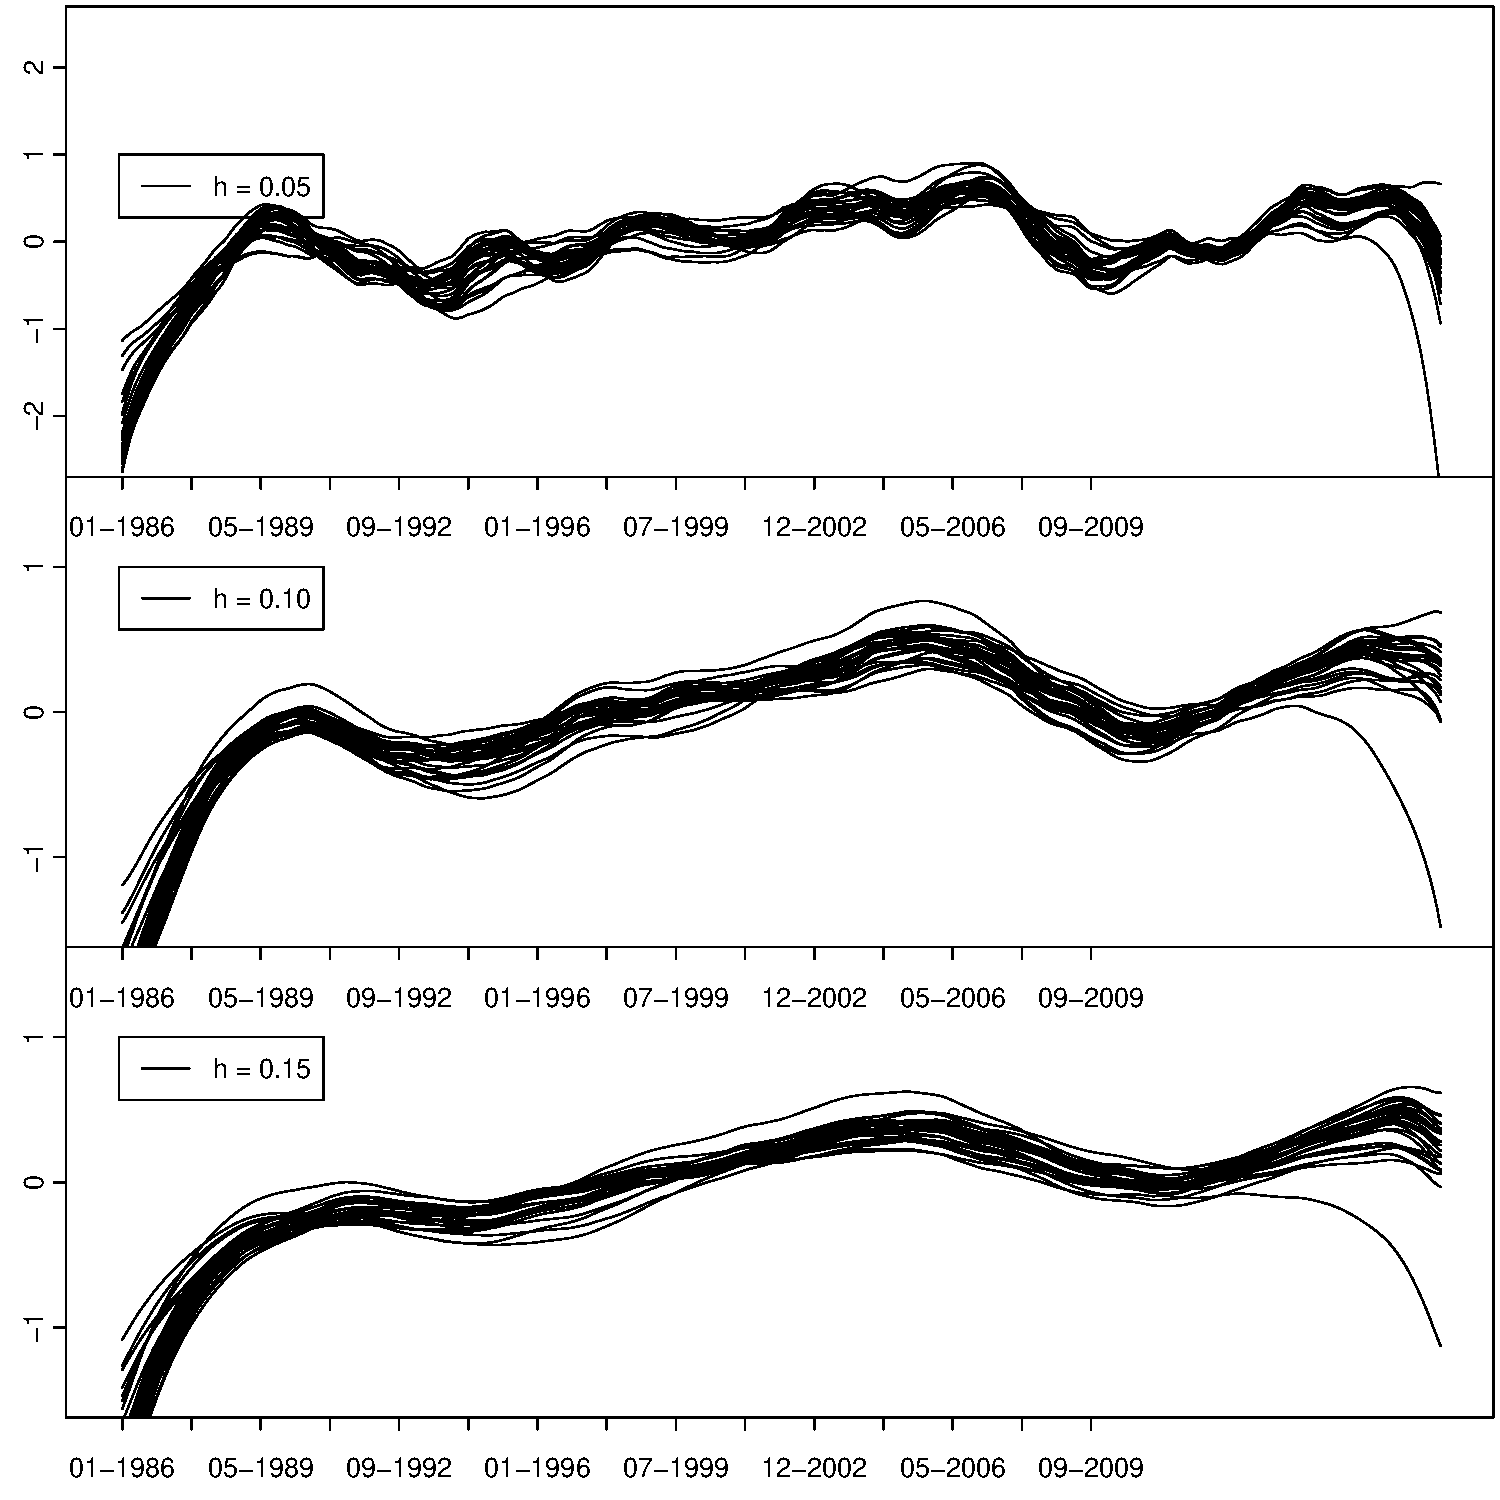
\includegraphics[width=0.8\textwidth]{Plots/stations_data.pdf}
%\vspace{0.2cm}
%\caption{Local linear kernel estimates of the $n=25$ time trends from the application of Section \ref{subsec-data-2}. Each panel shows the estimates for a different bandwidth $h$.}\label{plot-results-app2}
%\end{figure}


To illustrate our test method from Section \ref{sec-test-equality}, we examine a dataset of monthly mean temperatures from $34$ different UK weather stations. The data are publicly available on the webpage of the UK Met Office. We use a subset of $25$ stations for which data are available over the time span from $1986$ to $2017$. We thus observe a time series $\mathcal{Y}_i = \{Y_{it}: 1 \le t \le T \}$ of length $T = 386$ for each station $i \in \{1,\ldots,25\}$. The time series $\mathcal{Y}_i$ is assumed to follow the model 
\begin{equation}\label{model2-app}
Y_{it} = \alpha_i(t) + m_i\Big(\frac{t}{T}\Big) + \varepsilon_{it}, 
\end{equation}
where $m_i$ is an unknown nonparametric time trend and $\alpha_i(t)$ is a month-specific intercept which captures the seasonality pattern in the data. We suppose that $\alpha_i(t) = \alpha_i(t + 12 \ell)$ for any integer $\ell$, that is, we have a different intercept $\alpha_i(k)$ for each month $k = 1,\ldots,12$. The test method and the underlying theory from Section \ref{sec-test-equality} can be easily adapted to model \eqref{model2-app}, which is a slight extension of model \eqref{model2}. The details are provided below. As in Section \ref{subsec-data-1}, the error process $\mathcal{E}_i = \{ \varepsilon_{it}: 1 \le t \le T \}$ is assumed to have the AR(1) structure $\varepsilon_{it} = a_i \varepsilon_{i,t-1} + \eta_{it}$ for each $i$, where $\eta_{it}$ are i.i.d.\ innovations with mean zero.  


\newpage
\bibliographystyle{ims}
{\small
\setlength{\bibsep}{0.55em}
\bibliography{bibliography}}

\end{document}